\documentclass[tikz,border=15pt]{standalone}
\usepackage{amsmath}
\usetikzlibrary{shapes.geometric, arrows.meta, positioning, calc}

\begin{document}
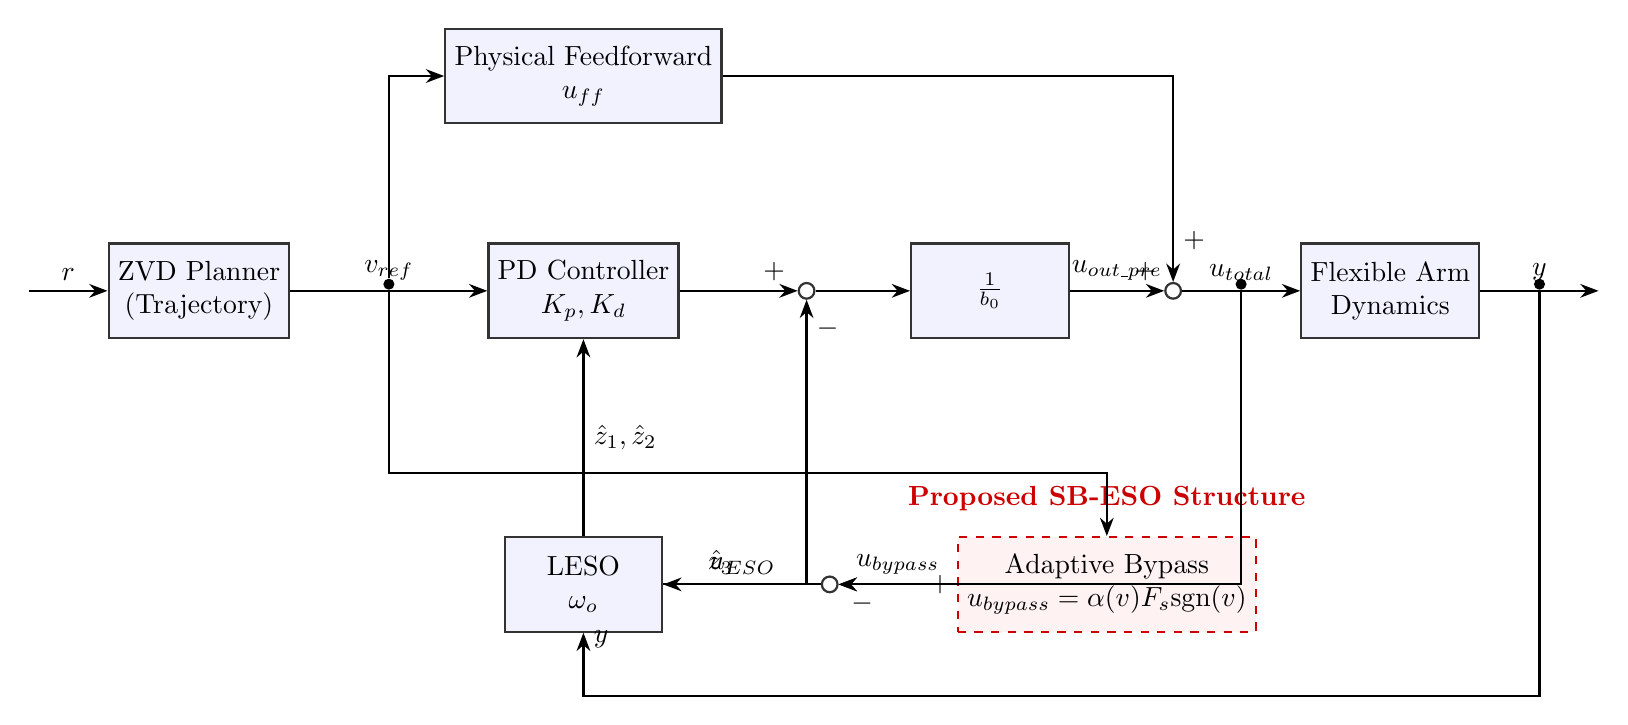
\begin{tikzpicture}[
    >=Stealth,
    auto,
    node distance=1.5cm and 2cm,
    % Standard Block Style
    block/.style={draw=black!80, rectangle, fill=blue!5, thick, minimum height=1.2cm, minimum width=2cm, align=center},
    % Summing Junction Style
    sum/.style={draw=black!80, circle, inner sep=2pt, thick},
    % Signal Branch Point Style
    branch/.style={fill, shape=circle, minimum size=4pt, inner sep=0pt},
    % Innovation Highlight Style (Red dashed)
    highlight/.style={draw=red!80!black, rectangle, fill=red!5, thick, dashed, minimum height=1.2cm, minimum width=2.5cm, align=center}
]

% ================= Nodes =================

% 1. Trajectory & Controller (Middle Row)
\node[coordinate] (ref) {};
\node[block, right=1cm of ref] (zvd) {ZVD Planner \\ (Trajectory)};
\node[block, right=2.5cm of zvd] (pd) {PD Controller \\ $K_p, K_d$};
\node[sum, right=1.5cm of pd] (sum_z3) {};
\node[block, right=1.2cm of sum_z3] (b0) {$\frac{1}{b_0}$};
\node[sum, right=1.2cm of b0] (sum_ff) {};

% 2. Plant (Middle Row)
\node[block, right=1.5cm of sum_ff] (plant) {Flexible Arm \\ Dynamics};
\node[coordinate, right=1.5cm of plant] (y_out) {};

% 3. Feedforward (Top Row)
\node[block, above=1.5cm of pd] (ff) {Physical Feedforward \\ $u_{ff}$};

% 4. ESO (Bottom Row)
\node[block, below=2.5cm of pd] (eso) {LESO \\ $\omega_o$};

% 5. Adaptive Bypass Innovation (Bottom Row)
\node[sum, right=2cm of eso] (sum_eso) {};
\node[highlight, right=1.5cm of sum_eso] (bypass) {Adaptive Bypass \\ $u_{bypass} = \alpha(v) F_s \text{sgn}(v)$};

% Label for the innovation
\node[above=0.2cm of bypass, text=red!80!black, font=\bfseries] {Proposed SB-ESO Structure};


% ================= Connections =================

% Main Forward Path
\draw[->, thick] (ref) -- node {$r$} (zvd);
\draw[->, thick] (zvd) -- coordinate[branch] (br_v) node[above] {$v_{ref}$} (pd);
\draw[->, thick] (pd) -- node[pos=0.8, above] {$+$} (sum_z3);
\draw[->, thick] (sum_z3) -- (b0);
\draw[->, thick] (b0) -- node {$u_{out\_pre}$} node[pos=0.8, above] {$+$} (sum_ff);
\draw[->, thick] (sum_ff) -- coordinate[branch] (br_u) node[above] {$u_{total}$} (plant);
\draw[->, thick] (plant) -- coordinate[branch] (br_y) node[above] {$y$} (y_out);

% Feedforward Path
\draw[->, thick] (br_v) |- (ff);
\draw[->, thick] (ff) -| node[pos=0.9, right] {$+$} (sum_ff);

% Innovation: Bypass Path
% Route velocity to bypass block
\draw[->, thick] (br_v) |- ($(bypass.north) + (0, 0.8)$) -- (bypass.north);
% Route total u to ESO summing junction
\draw[->, thick] (br_u) |- node[pos=0.9, right] {$+$} (sum_eso);
% Subtract bypass from u
\draw[->, thick] (bypass) -- node[above] {$u_{bypass}$} node[pos=0.8, below] {$-$} (sum_eso);
% Feed pure u to ESO
\draw[->, thick] (sum_eso) -- node[above] {$u_{ESO}$} (eso);

% ESO Feedback Paths
% Route y to ESO
\draw[->, thick] (br_y) |- ($(eso.south) - (0, 0.8)$) -| (eso.south) node[pos=0.95, right] {$y$};
% Route z3 to compensation junction
\draw[->, thick] (eso) -| node[pos=0.2, above] {$\hat{z}_3$} node[pos=0.95, right] {$-$} (sum_z3);
% Route z1, z2 to PD
\draw[->, thick] (eso) -- node[right] {$\hat{z}_1, \hat{z}_2$} (pd);

\end{tikzpicture}
\end{document}